\documentclass{article}
\usepackage{geometry}
\usepackage{graphicx}
\usepackage{enumerate}
\usepackage{amsmath}
\usepackage[utf8]{inputenc}
\usepackage[T1]{fontenc}
\usepackage[polish]{babel}

\author{Paulina Kukuła}            %preambuła
\date{12.12.2019} 
\title{Lab 8 - \LaTeX}


\begin{document}

\maketitle

\tableofcontents

\newpage

\section{Zadanie 3}
\subsection{Podpunkt a}

\vspace{0,5cm}

\hspace{0,5cm} \textsc{Mr. and Mrs. Dursley}, of number \textnormal{four}, \textbf{Privet Drive}, were proud to say that they were perfectly normal, \texttt{thank you very much}. They were the last people you'd expect to be involved in anything \emph{strange or mysterious}, because they just didn't hold with such \textit{nonsense}.
 
\vspace{0,5cm}
Mr. Dursley was the director of a firm called Grunnings, which made
drills. He was a big, beefy man with hardly any neck, although he did
have a very large mustache. Mrs. Dursley was thin and blonde and had
nearly twice the usual amount of neck, which came in very useful as she
spent so much of her time craning over garden fences, spying on the
neighbors. The Dursleys had a small son called Dudley and in their
opinion there was no finer boy anywhere.

\vspace{0,5cm}
The Dursleys had everything they wanted, but they also had a secret, and
their greatest fear was that somebody would discover it. They didn't
think they could bear it if anyone found out about the Potters. Mrs.
Potter was Mrs. Dursley's sister, but they hadn't met for several years;
in fact, Mrs. Dursley pretended she didn't have a sister, because her
sister and her good-for-nothing husband were as unDursleyish as it was
possible to be. The Dursleys shuddered to think what the neighbors would
say if the Potters arrived in the street. The Dursleys knew that the
Potters had a small son, too, but they had never even seen him. This boy
was another good reason for keeping the Potters away; they didn't want
Dudley mixing with a child like that.

\vspace{0,5cm}
When Mr. and Mrs. Dursley woke up on the dull, gray Tuesday our story
starts, there was nothing about the cloudy sky outside to suggest that
strange and mysterious things would soon be happening all over the
country. Mr. Dursley hummed as he picked out his most boring tie for
work, and Mrs. Dursley gossiped away happily as she wrestled a screaming
Dudley into his high chair.

\vspace{0,5cm}
None of them noticed a large, tawny owl flutter past the window.
At half past eight, Mr. Dursley picked up his briefcase, pecked Mrs.
Dursley on the cheek, and tried to kiss Dudley good-bye but missed,
because Dudley was now having a tantrum and throwing his cereal at the
walls. "Little tyke," chortled Mr. Dursley as he left the house. He got
into his car and backed out of number four's drive.

\vspace{0,5cm}
It was on the corner of the street that he noticed the first sign of
something peculiar — a cat reading a map. For a second, Mr. Dursley
didn't realize what he had seen — then he jerked his head around to
look again. There was a tabby cat standing on the corner of Privet
Drive, but there wasn't a map in sight. What could he have been thinking
of? It must have been a trick of the light. Mr. Dursley blinked and
stared at the cat. It stared back. As Mr. Dursley drove around the
corner and up the road, he watched the cat in his mirror.  \cite{harry}

\newpage
\section{Zadanie 4}
\vspace{0,3cm}
\subsection{Egzaminy}

\begin{enumerate}[\hspace{0,5cm}a)]
	\item Bazy danych
	\item Podstawy ochrony danych
	\item Grafika komputerowa i komunikacja człowiek komputer
\end{enumerate}

\vspace{0,3cm}
\subsection{Języki programowania}

\begin{itemize}
	\item Java
	\item C++
	\item C
	\item Python
\end{itemize}

\vspace{1cm}
\section{Zadanie 5}
\vspace{0,3cm}
\subsection{Cudzysłowy}
\vspace{0,5cm}
Tu powinien być cytat od kolegi, ale nie wiem co dać do bibliografii, więc dam tu cytat z książki, żeby móc potem podać jego źródło: "But you know, happiness can be found even in the darkest of times, if one only remembers to turn on\footnote{zapalić} the light". \cite{cyt}




\newpage
\section{Zadanie 6}
\vspace{0,3cm}
\subsection{Rysunek}

\begin{figure}[h]                % h - here!
	\centering
	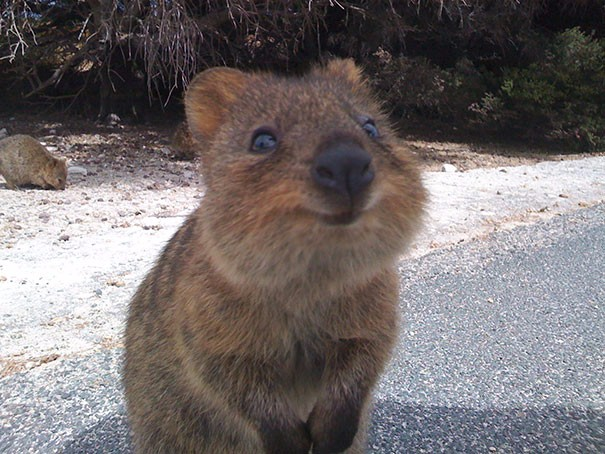
\includegraphics[height=8cm]{kuoka.jpg}
	\caption{Bardzo radosna kuoka}
	\label{kuoka}
\end{figure}


\subsection{Tabela}
\vspace{0,3cm}

\begin{table}[h]
	
	\centering
	\caption{Przykładowe województwa}
	\vspace{0,2cm}
	\label{tabela}
	
	\begin{tabular}{ | c | c | c |}
		\hline
		\textbf{Województwo} & \textbf{Powierzchnia} & \textbf{Populacja} \\ [0.5ex] 
		\hline\hline
		wielkopolskie & 29 826,50 & 3 493 969 \\ 
		\hline
		pomorskie & 18 310,34 & 2 333 523	 \\  
		\hline
		dolnośląskie & 19 946,70 & 2 901 225 \\
		\hline 
	\end{tabular}

\end{table}

\begin{center}
	Kuoka na rysunku \ref{kuoka} jest śliczna!
	Tabela jest umieszczona na stronie \pageref{tabela}.
\end{center}

\begin{center}
	W otoczeniu tabular szerokosc poszczególnych kolumn tabeli jest ustalana
	automatycznie, a szerokosc tabeli jest suma szerokosci kolumn i odstepów
	miedzykolumnowych. \cite{lat}
\end{center}



\newpage
\section{Zadanie 7}
\vspace{0,3cm}
\subsection{Równania}

\begin{enumerate}[\hspace{0,5cm}a)]
	
	\item 
	\begin{equation*}
	\Big(
		\begin{matrix}
		n \\ k
		\end{matrix}
	\Big) = \frac{n!}{k!(n-k)!}
	\end{equation*}
	
	\item 
	\begin{equation*}
	a^2 + b^2 = c^2
	\end{equation*}
	
	\item 
	\begin{equation*}
	\frac{ \frac{1}{2} + \frac{1}{4}} {\frac{1}{8}} \neq 1
	\end{equation*}
	
	\item 
	\begin{equation*}
	\sum_{i=1}^{n} i^2 = \frac{ n(n+1)(2n+1 )} {6}
	\end{equation*}
	
	\item 
	\begin{equation*}
	C_{2}^{-3} + O_{2}^{0} \rightarrow C^{+4}O_{2}^{-2} + H_{2}^{+1}O^{-2}
	\end{equation*}

	\item 
	\begin{equation*}
	A_{m,n} = 
	\left\lgroup
		\begin{matrix}
			a_{1,1} & a_{1,2} & \cdots & a_{1,n}  \\ 
			a_{2,1} & a_{2,2} & \cdots & a_{2,n}  \\ 
			\vdots & \vdots & \ddots & \vdots     \\ 
			a_{m,1} & a_{m,2} & \cdots & a_{m,n}  \\  
		\end{matrix}
	\right\rgroup
	\end{equation*}

\end{enumerate}


\vspace{1cm}
\section{Bibliografia}
\bibliographystyle{plain}
\bibliography{bibliografia} 


\end{document}


\begin{comment}

 Każdy plik źródłowy składa się z dwóch części: preambuły oraz części głównej. 
 
 Preambuła powinna się rozpoczynać od instrukcji:\documentclass{...}
 Polecenie to okresla typ tworzonego dokumentu. Po nim można umieścić instrukcje dotyczące stylu całego dokumentu oraz dołączyć pakiety poszerzające możliwości LaTeXa. Pakiety dołącza się za pomocą polecenia:\usepackage{...}

 Część główna dokumentu zaczyna się od instrukcji \begin{document}, a kończy poleceniem \end{document}. Tekst znajdujący się za tym poleceniem jest przez LaTeX-a ignorowany.
 
 
\end{comment}




